\documentclass[a4paper,onecolumn,12pt]{article}

\usepackage[czech]{babel}
\usepackage[utf8]{inputenc}
\usepackage[left=2.5cm,right=2.5cm,top=2.5cm,bottom=2.5cm]{geometry}
\usepackage{graphicx}   


% pro specifikaci formátu datumu
\usepackage{datetime}
\newdateformat{czdate}{\THEDAY.\THEMONTH.\:\THEYEAR}
% použití: \czdate\today

% definice zadani
\newenvironment{zadani}
{\begin{center}\textbf{Zadání:}\itshape}{\end{center}}

% odstavce
\usepackage{parskip}

%====== Units =====
\usepackage{siunitx}
\sisetup{inter-unit-product =\ensuremath{\cdot}}
\sisetup{group-digits = integer}
\sisetup{group-minimum-digits = 4}
\sisetup{group-separator=\,}
\sisetup{output-decimal-marker = {,}}
\sisetup{exponent-product = \ensuremath{\cdot}}
\sisetup{separate-uncertainty}
\sisetup{tight-spacing = false}
%\sisetup{scientific-notation = true}
%\sisetup{round-mode=places,round-precision=4}
%\sisetup{evaluate-expression}


% Boltzmannova konstanta
\newcommand{\constkval}{\num{1.38e-23}}
\newcommand{\constkunit}{\unit{\joule\per\kelvin}}

% Planckova konstanta
\newcommand{\consthval}{\num{6.626e-34}}
\newcommand{\consthunit}{\unit{\joule\second}}

% Rychlost světla
\newcommand{\constcval}{\num{2.998e8}}
\newcommand{\constcunit}{\unit{\meter\per\second}}

% Elementární náboj
\newcommand{\consteval}{\num{1.602e-19}}
\newcommand{\consteunit}{\unit{\coulomb}}

% Hmotnost elektronu
\newcommand{\constmeval}{\num{9.109e-31}}
\newcommand{\constmeunit}{\unit{\kilogram}}

% align bloky rovnic
\usepackage{amsmath}

\begin{document}
\setlength{\textwidth}{\paperwidth-5cm}
\title{Samostatná práce II – BPC-EMV2}
\author{Jakub Charvot}
\date{\czdate\today}
\maketitle

\section*{Úvod}

V této práci jsou prezentovány výpočty z oblasti elektronových procesů, iontových procesů, rentgenových procesů, jaderných procesů, laserových procesů a ultraakustických procesů.


% Elektronove procesy
\section{Elektronové procesy}

\subsection{Přehled elektronových procesů}

Elektronové procesy jsou procesy, při kterých jsou zapojeny elektrony. Tyto procesy mohou být popsány pomocí různých metod, např. Bornovy aproximace nebo Hartreeho-Fockovy metody.

\subsection{Příklad 1.1.2 - výpočet}
\begin{zadani}
    Určete hustotu emisního proudu rozžhaveného wolframového vlákna 
    při teplotě 2 227 °C , působí-li současně elektrické pole o intenzitě 
    E = 2.105 V.m-1
\end{zadani}

Nejprve je potřeba vypočítat emisní proud samotného vlákna, k tomu slouží následující vztah:
\[
    j_{eT} = A T^2 \exp\left(-\frac{W}{kT}\right)
\]
Po dosazení dostáváme:
\[
    j_{eT} =\qty{3155}{\ampere\per\square\meter}
\]
Takto vypočtená hodnota odpovídá emisnímu proudu samotného wolframového vlákna, bez působení el. pole. Působením napětí můžeme proudovou hustotu výrazně zesílit, platí zde následující vztah:
\begin{align*}
    j_{eTE} &= A T^2 \exp\left(-\frac{W-\Delta W}{kT}\right) \\
    j_{eTE} &= A T^2 \exp\left(-\frac{W}{kT}\right) \cdot \exp\left(\frac{\Delta W}{kT}\right) \\
    j_{eTE} &= j_{eT} \cdot \exp\left(\frac{\Delta W}{kT}\right)= j_{eT} \cdot \exp\left(\frac{0,44\sqrt{E} }{T}\right)\\
    j_{eTE} &= \num{3155}\exp\left(\frac{0,44\sqrt{\num{2e5}} }{\num{2500}}\right) \\
    j_{eTE} &= \qty{3413}{\ampere\per\square\meter }
\end{align*}



\subsection{Příklad 1.1.3 - výpočet}
\begin{zadani}
    Určete emisní proud katody vyrobené ve tvaru disku o průměru 10 mm
    z wolframu, vyhřáté na teplotu 2 227 oC. Urychlovací anoda je umístěna 
    ve vzdálenosti  50 mm  od katody a je na ni přivedeno napětí  10 kV
\end{zadani}

Vyjdete z proudové hustoty vypočtené v předchozím příkladu, pro stanovení proudu stačí stanovit plochu katody a dosadit do obecně známého vztahu:

\begin{align*}
  I&=j_{eTE} S = j_{eTE} \frac{\pi d^2}{4}\\
  I&=j_{eTE} S = \num{3413} \frac{\pi (\num{10e-3})^2}{4}\\
  I&=\qty{0.268}{\ampere}
\end{align*}



% Iontove procesy
\section{Iontové procesy}

\subsection{Příklad 1.2.1}
\begin{zadani}
    Srovnejte základní vlastnosti elektronů a iontů.
\end{zadani}

Elektrony mají vždy záporný náboj a jsou obecně podstatně lehčí a menší než ionty. Díky své nízké hmotnosti se mohou pohybovat velmi vysokými rychlostmi blížícími se rychlosti světla. 

Ionty mohou mít kladný i záporný náboj a jsou větší a těžší. Oproti elektronům mohou také tvořit chemické reakce (jelikož se jedná o celé ionizované atomy nebo molekuly). Lze je použít například i pro depozici tenkých vrstev.


\subsection{Příklad 1.2.2 - výpočet}
\begin{zadani}
    Stanovte maximální koncentraci implantovaných iontů bóru do 
    monokrystalu křemíku ve vzdálenosti středního doletu iontů  Rp od 
    povrchu destičky a koncentraci iontů ve vzdálenosti  Rp \(\pm \Delta\)Rp a na 
    povrchu monokrystalu.  \(\Delta\)Rp  je střední kvadratická odchylka. Zjištěný  
    koncentrační profil naznačte graficky. Celková dávka  Q = 1018 m-2 při  
    energie iontů  100 keV
\end{zadani}


Pro implantaci bóru do křemíku při energii iontů \qty{100}{keV} platí:

Rp = \qty{0,2994}{\micro\meter} a \(\Delta\)Rp = \qty{0,0710}{\micro\meter}

Pro stanovení maximální koncentrace vyjdeme z následujícího vztahu:
\begin{align*}
  N_{max} &= \frac{Q}{\sqrt{2\pi \Delta R_{p} } } \\
  N_{max} &= \frac{\num{10e18}}{\sqrt{2\pi \num{0,0710e-6} } } \\
  N_{max} &= \qty{1,49e21}{\per\meter\cubed}
\end{align*}

Jak by vypadal koncentrační profil v závislosti na vzdálenosti od povrchu můžeme vidět na obrázku~\ref{fig:img-profil}

\begin{figure}[h!]
  \centering
  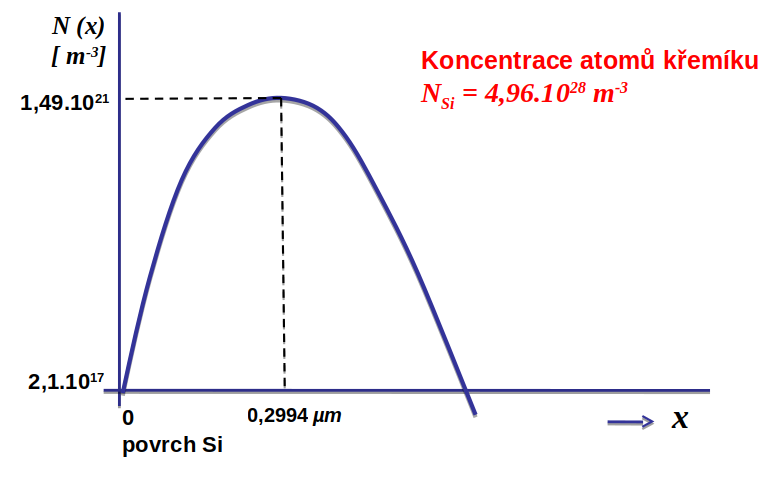
\includegraphics[width=0.6\textwidth]{img/profil.png}
  \caption{Závislost koncentrace dopantů na hloubce resp. vzdálenosti od povrchu.}
  \label{fig:img-profil}
\end{figure}



% Rentgenove procesy
\section{Rentgenové procesy}

\subsection{Přehled rentgenových procesů}

Rentgenové procesy jsou procesy, při kterých jsou zapojeny rentgenové záření. Tyto procesy mohou být popsány pomocí různých metod, např. Bornovy aproximace nebo Hartreeho-Fockovy metody.

\subsection{Příklad 2.1.1 - výpočet}
\begin{zadani}
    Stanovte nejkratší vlnovou délku rentgenového záření vzniklého 
    po dopadu svazku elektronů na kov. Urychlovací napětí  U = 2 kV
\end{zadani}


Nejkratší vlnovou délku bude mít záření s nejvyšší energií, musíme tedy stanovit maximální energii dopadajících elektronů. Ty jsou urychlovány napětím \(U\), bude to tedy vypadat takto:
\begin{align*}
  \lambda_{min} &=\frac{hc}{E}=\frac{hc}{qU} \\
  \lambda_{min} &=\frac{\consthval\cdot\constcval}{\consteval\cdot \num{2e3}}\\
  \lambda_{min} &= \qty{0,619}{nm}
\end{align*}


\subsection{Příklad 2.1.2 - výpočet}
\begin{zadani}
    Stanovte vlnovou délku rentgenového záření pro kterou dosáhne 
    intenzita záření maxima. Urychlovací napětí  U = 2 kV
\end{zadani}


Ze spektrální charakteristiky vyzářeného rtg. záření bylo empiricky zjištěno, že maximální intenzita záření odpovídá frekvenci, při které má záření energii připbližně 0,6 maximální hodnoty. Upravíme tedy výpočet:

\begin{align*}
    \lambda_{I_{max}} &=\frac{hc}{0,6E}=\frac{hc}{0,6qU} \\
    \lambda_{I_{max}} &=\frac{\consthval\cdot\constcval}{0,6\consteval\cdot \num{2e3}}\\
    \lambda_{I_{max}} &= \qty{1,032}{nm}
  \end{align*}



% Jaderné procesy
\section{Jaderné procesy}

\subsection{Přehled jaderných procesů}

Jaderné procesy jsou procesy, při kterých jsou zapojena jádra atomů. Tyto procesy mohou být popsány pomocí různých metod, např. Bornovy aproximace nebo Hartreeho-Fockovy metody.

\subsection{Příklad 2.2.1 - výpočet}
\begin{zadani}
    Stanovte rychlost s jakou se pohybují  tzv. tepelné neutrony
    při teplotě 25 °C 
\end{zadani}

Vyjdeme zde z kinetické energie neutronu, ta je rovna jeho energii tepelné:
\[
    E=\frac{1}{2}m_{n} v_{n}^{2}=kT 
\]
Z této rovnosti vyjádříme rychlost neutronu v závislosti na termodynamické teplotě:
\begin{align*}
  v_{n} &= \sqrt{\frac{2kT}{m_{n}}} \\ 
  v_{n} &= \sqrt{\frac{2\constkval(25+273,15)}{\num{1,674e-27}}} \\ 
  v_{n} &= \qty{2216}{\meter\per\second}
\end{align*}


\subsection{Příklad 2.2.7 - výpočet}
\begin{zadani}
    Stanovte kolikrát se zmenší tok tepelných neutronů při průchodu
    destičkou z kadmia a hliníku o tloušťce 1 mm. Účinný průřez pro
    kadmium  \(\sigma_{Cd} \)= 2 500.10-28 m2  a pro hliník  \(\sigma_{Al} \)= 0,21.10-28 m2 
\end{zadani}

Pro vypočtení tohoto příkladu je potřeba stanovit absorbční koeficient obou materiálů:
\begin{align*}
    \alpha &= n\sigma \\\\
    \alpha_{Cd}  &= n_{Cd} \sigma_{Cd} = \num{4,6e28}\cdot \num{2500e-28}= \qty{11500}{\per\meter}\\
    \alpha_{Al}  &= n_{Al} \sigma_{Al} = \num{6,02e28}\cdot \num{0,21e-28}= \qty{1,26}{\per\meter}
\end{align*}

Následně využijeme vztah pro stanovení toku neutronů po průchodu vrstvou materiálu tlustou x m:
\begin{align*}
    \varphi(x) &= \varphi_{0} \cdot \exp(-\alpha x)\\
    \frac{\varphi_{0}}{\varphi(x)} &=\frac{1}{\exp(-\alpha x)}
\end{align*}

Zlomek na posledním řádku přímo odpovídá na naši otázku "kolikrát se zmenší?". Po dosazení hodnot pro oba materiály získáme následující hodnoty:
\begin{itemize}
    \item Po průchodu kadmiem se tok zmenší \num{99009} krát. 
    \item Po průchodu hliníkem pouze \num{1,002} krát.
\end{itemize}





% Laserove procesy
\section{Laserové procesy}

\subsection{Příklad 3.1.1 - výpočet}
\begin{zadani}
    Yttrium-Aluminium-Granát laser dotovaný neodymem, YAG:Nd3+, 
    má rozdíl energií mezi horní a spodní laserovou hladinou 1,17 eV. 
    Určete vlnovou délku příslušného laserového záření a stanovte
    jaké oblasti spektra odpovídá.
\end{zadani}


Energie vyzářeného fotonu je přímo svázaná s vlnovou délkou takového záření:
\begin{align*}
  \lambda &= \frac{hc}{\Delta E} \\
  \lambda &= \frac{\consthval\constcval}{1,17\cdot \consteval} \\
  \lambda &= \qty{1,06e-6}{\meter}
\end{align*}

Tato vlnová délka odpovídá infračervené oblasti elektromagnetického spektra.


\subsection{Příklad 3.1.4 - výpočet}
\begin{zadani}
    Laserový svazek o průměru d = 0,1 mm  dopadl kolmo na destičku z
    křemíku. Výkon přenášený ve svazku je P = 10 kW.  Stanovte plošnou 
    hustotu výkonu laserového záření po průchodu destičkou o tloušťce 
    x = 2 mm,  použijeme-li záření o vlnové délce \(\lambda\)  = 1,06 µm, součinitel 
    reflexe uvažujme  R = 0,28  a absorpční součinitel \(\alpha(\lambda)\)  = 5 cm-1.
   Rozhodněte, zda na dané vlnové délce lze křemík použít pro optické 
    systémy
\end{zadani}


Zde se kombinují dva jevy, nejprve se část intenzity paprsku odrazí zpět a následně je část pohlcena materiálem. Pro stanovení hustoty výkonu po průchodu systémem musíme zohlednit oba jevy. 

Plošná hustota výkonu na začátku:
\[
    N_{S_{0} } =\frac{P_{0}}{S}=\frac{4P_{0}}{\pi d^2} = \qty{1,27e12}{\watt\per\square\meter} 
\]
Odečtení odraženého výkonu: 
\[
    N_{S_{0} }^\prime = N_{S_{0} } (1-R)=\qty{9,144e11}{\watt\per\square\meter}
\]
Odečtení absorbovaného výkonu: 
\begin{align*}
  N_{S} &= N_{S_{0} }^\prime\cdot \exp(-\alpha(\lambda)x) \\
  N_{S} &= \num{9,144e11}\cdot \exp(-\num{5e2}\cdot \num{2e-3}) \\
  N_{S} &= \qty{3,36e11}{\watt\per\square\meter}
\end{align*}
 


% Ultraakustické procesy
\section{Ultraakustické procesy}

\subsection{Přehled ultraakustických procesů}

Ultraakustické procesy jsou procesy, při kterých jsou zapojeny zvukové vlny. Tyto procesy mohou být popsány pomocí různých metod, např. Bornovy aproximace nebo Hartreeho-Fockovy metody.

\subsection{Příklad 3.2.4 - výpočet}
\begin{zadani}
    Jak velký výkon bude předán destičce o ploše 1 cm2 ponořené ve 
    vodě, bude-li amplituda kmitů Y = 10-6 m  při kmitočtech 20 kHz a 
    1 MHz, při kolmém dopadu a úplné absorpci vlnění?
\end{zadani}


Výkon akustických vln závisí na prostředí, kde vlna působí (to určuje rychlost šíření vlnění) a také jeho amplituda. Výkon označíme \(P\) a vyjdeme z následujícího vztahu:
\begin{align*}
    P &= \frac{1}{2}\omega^2 Y^2 \rho vS
\end{align*}
Dosazení pro \qty{20}{kHz}:
\begin{align*}
    P &= \frac{1}{2}(2\pi\cdot \num{20e3})^2 (\num{e-6})^2 \num{1000}\cdot \num{1483}\cdot \num{1e-4} \\
    P &= \qty{1,17}{\watt} \\
\end{align*}
Dosazení pro \qty{1}{MHz}:
\begin{align*}
    P &= \frac{1}{2}(2\pi\cdot \num{1e6})^2 (\num{e-6})^2 \num{1000}\cdot \num{1483}\cdot \num{1e-4} \\
    P &= \qty{2,926}{\kilo\watt} \\
\end{align*}

\subsection{Příklad 3.2.7 - výpočet}
\begin{zadani}
    Vypočtěte jak velká část intenzity dopadajícího ultrazvukového vlnění 
    projde do oceli a jak velká část se odrazí při kolmém dopadu 
    akustické vlny na rozhraní  voda – ocel,  resp.  vzduch – ocel
\end{zadani}


Pro rozhraní libovolných dvou prostředí lze stanovit součinitel odrazu, který udává, jak velká část intenzity vlnění se odrazí zpět, zbytek naopak projde. 
Tento součinitel závisí na akustickém vlnovém odporu obou prostředí. 

Výpočet akustického vlnového odporu:
\[
    Z_{a} = \rho v
\]
\begin{align*}
  \text{Vz}&\text{duch:} & \text{Vo}&\text{da:} & \text{Oc}&\text{el:} \\
  Z_{vz} &= \rho_{vz} v_{vz} & Z_{vo} &= \rho_{vo} v_{vo} & Z_{oc} &= \rho_{oc} v_{oc} \\
  Z_{vz} &= \num{1,276}\cdot\num{332} & Z_{vo} &= \num{1000}\cdot\num{1483} & Z_{oc} &= \num{7800}\cdot\num{6000} \\
  Z_{vz} &= \qty{423.6}{\kilo\gram\per\square\meter\per\second} & Z_{vo} &= \qty{1.483e6}{\kilo\gram\per\square\meter\per\second} & Z_{oc} &= \qty{4.68e7}{\kilo\gram\per\square\meter\per\second} \\
\end{align*}

Koeficienty odrazu:
\begin{align*}
  R_{vo-oc} &= \left( \frac{Z_{vo}-Z_{oc}}{Z_{vo}+Z_{oc}} \right)^2 \\
  R_{vo-oc} &= \left( \frac{\num{1,483e6}-\num{4,68e7}}{\num{1,483e6}+\num{4,68e7}} \right)^2 \\
  R_{vo-oc} &= \num{0,881} = \qty{88,1}{\percent}  
\end{align*}
Na rozhraní voda--ocel se odrazí \qty{88,1}{\percent} intenzity vlnění, zbylých \qty{11,9}{\percent} projde dále.

\begin{align*}
    R_{vo-oc} &= \left( \frac{Z_{vz}-Z_{oc}}{Z_{vz}+Z_{oc}} \right)^2 \\
    R_{vo-oc} &= \left( \frac{\num{423,6}-\num{4,68e7}}{\num{423,6}+\num{4,68e7}} \right)^2 \\
    R_{vo-oc} &= \num{1} = \qty{100}{\percent}  
\end{align*}
Na rozhraní vzduch--ocel se odrazí téměř \qty{100}{\percent} intenzity vlnění.



\section*{Závěr}

V této práci byly prezentovány výpočty z oblasti elektronových procesů, iontových procesů, rentgenových procesů, 
jaderných procesů, laserových procesů a ultraakustických procesů. Pro každou oblast byly uvedeny příklady a provedeny výpočty s použitím různých metod. Výsledky těchto výpočtů byly uvedeny v příslušných sekcích.

Výpočty byly provedeny s ohledem na principy dané oblasti a s použitím vhodných metod. Výsledky ukázaly, že metoda použitá k výpočtu může mít významný vliv na výsledky a jejich správnost.

Tato práce by mohla být rozšířena o další příklady a oblasti, a tím poskytnout více informací o různých procesech. Zároveň by bylo možné věnovat se více srovnání různých metod a zhodnocení, která metoda je pro danou oblast nejvhodnější.



\end{document}


